\documentclass{article}

\newcommand{\dir}{~/projects/latex} % IMPORTANT: No trailing slashes!
\input{\dir/include.tex}
\load{recommended}
\usetikzlibrary{automata, positioning, arrows.meta}
\newcommand{\hdelta}{\hat{\delta}}
\newcommand{\qacc}{q_{\text{accept}}}
\newcommand{\qrej}{q_{\text{reject}}}

\setup{Theoretical Computer Science - Compact}

\begin{document}
\startDocument
\usetcolorboxes


\section{Introduction}
This summary aims to provide a simple, easy to understand and short overview over the topics covered, with approaches for proofs, important theorems and lemmas,
as well as definitions.

It does not aim to serve as a full replacement for the book or my main summary, but as a supplement to both of them.

It also lacks some formalism and is only intended to give some intuition


\newsection
\section{Alphabets, Words, etc}
\stepcounter{subsection}
\subsection{Alphabets, Words, Languages}
\fancydef{Alphabet} Set $\Sigma$.
Important alphabets: $\alphabetbool$, $\alphabets{lat}$ (all latin chars), $\alphabets{Keyboard}$ (all chars on keyboard), $\Sigma_m$ ($m$-ary numbers)

\fancydef{Word} Possibly empty (denoted $\lambda$) sequences of characters from $\Sigma$. $|w|$ is the length, 
$\Sigma^*$ is the set of all words and $\Sigma^+ = \Sigma^* - \{ \lambda \}$

\fancydef{Konkatenation} $\text{Kon}(x, y) = xy$, (so like string concat). $(xy)^n$ is $n$-times repeated concat.

\fancydef{Reversal} $a^R$, simply read the word backwards.

\stepLabelNumber{definition}
\fancydef{Prefix, Suffix, Subword} $v$ in $w = vy$; $s$ in $w = sx$; Subword is $u$ in $w = xuy$

\fancydef{Appearance} $|x|_a$ is the number of times $a \in \Sigma$ appears in $x$

\fancydef{Canonical ordering} Ordered by length and then by first non-common letter:
\rmvspace
\begin{align*}
    u < v \Longleftrightarrow |u| < |v| \lor (|u| = |v| \land u = x \cdot s_i \cdot u' \land v = x \cdot s_j \cdot v') \text{ for any } x, u', v' \in \word \text{ and } i < j
\end{align*}

\drmvspace
\fancydef{Language} $L \subseteq \word$, and we define $L^C = \word - L$ as the complement, with $L_{\emptyset}$ being the empty language, 
whereas $L_\lambda$ is the language with just the empty word in it.

\bi{Concatenation}: $L_1 \cdot L_2 = \{ vw | v \in L_1 \land w \in L_2 \}$ and $L^{i + 1} = L^i \cdot L \ \forall i \in \N$.

\bi{Cleen Star}: $L^* = \bigcup_{i \in \N} L^i$ and $L^+ = L \cdot L^*$


\inlinelemma $L_1L_2 \cup L_1 L_2 = L_1(L_2 \cup L_3)$
\inlinelemma $L_1(K_2 \cap L_3) \subseteq L_1 L_2 \cap L_1 L_3$


\stepcounter{subsection}
\subsection{Kolmogorov-Complexity}
\setLabelNumber{definition}{17}
\fancydef{Kolmogorov-Complexity} $K(x)$ for $x \in \wordbool$ is the minimum of all binary lengths of Pascal programs that output $x$, 
where the Program doesn't have to compile, i.e. we can describe processes informally

\stepLabelNumber{lemma}
\inlinelemma For each word $x$ exists constant $d$ s.t. $K(x) \leq |x| + d$, for which we can use a program that simply includes a \texttt{write(x)} command

\fancydef{Of natural number} $K(n) = K(\text{Bin}(x))$ with $|\text{Bin}(x)| = \ceil{\log_2(x + 1)}$

\inlinelemma For each $n \in \N \exists w_n \in (\alphabetbool)^n$ s.t. $K(w_n) \geq |w_n| = n$, i.e. exists a non-compressible word.

\inlinetheorem Kolmogorov-Complexity doesn't depend on programming language. It only differs in constant

\fancydef{Randomness} $x$ random if $K(x) \geq |x|$, thus for $n$, $K(n) \geq \ceil{\log_2(n + 1)} - 1$

\stepLabelNumber{theorem}
\fancytheorem{Prime number} $\displaystyle \limni \frac{\text{Prime}(n)}{\frac{n}{\ln(n)}}$

\newsection
\section{Finite Automata}
\stepcounter{subsection}
\subsection{Representation}
We can note the automata using graphical notation similar to graphs or as a series of instructions like this:
\rmvspace
\begin{align*}
    \texttt{select } input & = a_1 \texttt{ goto } i_1 \\[-0.2cm]
    \vdots                                             \\
    input                  & = a_k \texttt{ goto } i_k
\end{align*}

\drmvspace
\fancydef{Finite Automaton}
\drmvspace
\begin{multicols}{2}
    \begin{itemize}
        \item $Q$ set of states
        \item $\Sigma$ input alphabet
        \item $\delta(q, a) = p$ transition from $q$ on reading $a$ to $p$
        \item $q_0$ initial state
        \item $F \subseteq Q$ accepting states
        \item $\mathcal{L}_{EA}$ regular languages (accepted by FA)
    \end{itemize}
\end{multicols}

\drmvspace
$\hat{\delta}(q_0, w) = p$ is the end state reached when we process word $w$ from state $q_0$, and $(q, w) \bigvdash{M}{*} (p, \lambda)$ is the formal definition,
with $\bigvdash{M}{*}$ representing any number of steps $\bigvdash{M}{}$ executed.

The class $\class[q_i]$ represents all possible words for which the FA is in this state.
Be cautious when defining them, make sure that no extra words from other classes could appear in the current class, if this is not intended.

Sometimes, we need to combine two (or more) FA to form one larger one.
We can do this easily with product automata. To create one from two automata $M_1$ (states $q_i$) and $M_2$ (states $p_j$) we do the following steps:
\rmvspace
\begin{enumerate}[noitemsep]
    \item Write down the states as tuples of the form $(q_i, p_j)$ (i.e. form a grid by writing down one of the automata vertically and the other horizontally)
    \item From each state, the automata on the horizontal axis decides for the input symbol if we move left or right,
          whereas the automata on the vertical axis decides if we move up or down.
\end{enumerate}

\begin{center}
    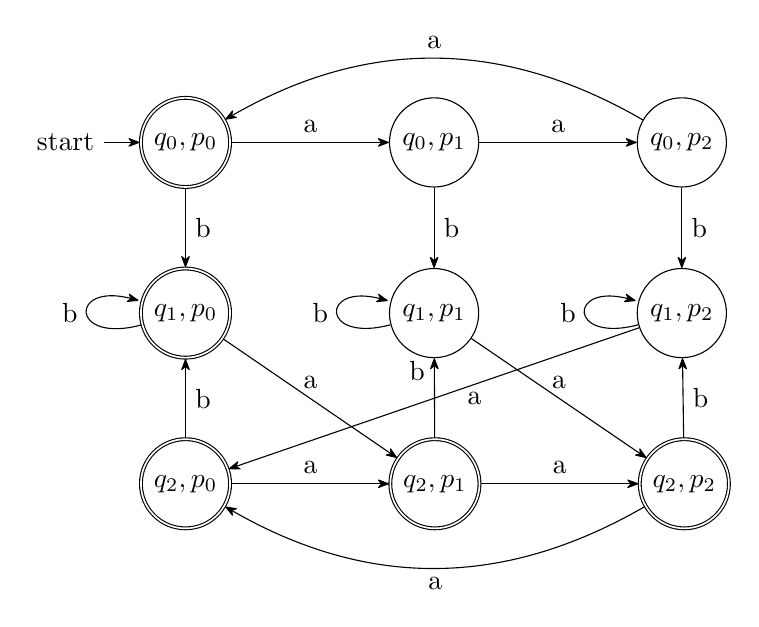
\begin{tikzpicture}[node distance = 1cm and 2cm, >={Stealth[round]}]
        \node[state, initial left, accepting] (q0p0) {$q_0, p_0$};
        \node[state] (q0p1) [right=of q0p0] {$q_0, p_1$};
        \node[state] (q0p2) [right=of q0p1] {$q_0, p_2$};
        \node[state, accepting] (q1p0) [below=of q0p0] {$q_1, p_0$};
        \node[state] (q1p1) [right=of q1p0] {$q_1, p_1$};
        \node[state] (q1p2) [right=of q1p1] {$q_1, p_2$};
        \node[state, accepting] (q2p0) [below=of q1p0] {$q_2, p_0$};
        \node[state, accepting] (q2p1) [right=of q2p0] {$q_2, p_1$};
        \node[state, accepting] (q2p2) [right=of q2p1] {$q_2, p_2$};

        \path[->]
        % Level 0
        (q0p0) edge node [above] {a} (q0p1)
        (q0p1) edge node [above] {a} (q0p2)
        (q0p2) edge [bend right] node [above] {a} (q0p0)
        % Level 0 to level 1
        (q0p0) edge node [right] {b} (q1p0)
        (q0p1) edge node [right] {b} (q1p1)
        (q0p2) edge node [right] {b} (q1p2)
        % Level 1 to level 2
        (q1p0) edge node [above] {a} (q2p1)
        (q1p1) edge node [above] {a} (q2p2)
        (q1p2) edge node [right, xshift=0.3cm] {a} (q2p0)
        % Level 2 to level 1
        (q2p0) edge node [right] {b} (q1p0)
        (q2p1) edge node [above left, yshift=0.1cm] {b} (q1p1)
        (q2p2) edge node [right] {b} (q1p2)
        % Level 2
        (q2p0) edge node [above] {a} (q2p1)
        (q2p1) edge node [above] {a} (q2p2)
        (q2p2) edge [bend left] node [below] {a} (q2p0)
        % ────────────────────────────────────────────────────────────────────
        % Loops on level 1
        (q1p0) edge [loop left] node {b} ()
        (q1p1) edge [loop left] node {b} ()
        (q1p2) edge [loop left] node {b} ();
    \end{tikzpicture}
\end{center}

For the automata
\begin{figure}[h!]
    \begin{subfigure}{0.49\textwidth}
        \begin{center}
            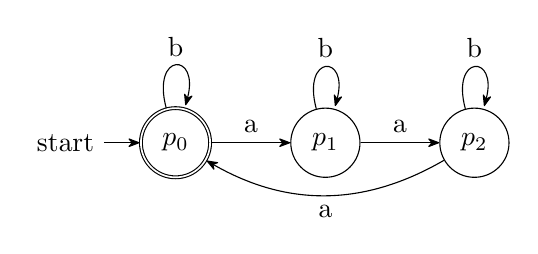
\begin{tikzpicture}[node distance = 1cm, >={Stealth[round]}]
                \node[state, initial left, accepting] (p_0) {$p_0$};
                \node[state] (p_1) [right=of p_0] {$p_1$};
                \node[state] (p_2) [right=of p_1] {$p_2$};

                \path[->]
                (p_0) edge node [above] {a} (p_1)
                (p_1) edge node [above] {a} (p_2)
                (p_2) edge [bend left] node [below] {a} (p_0)
                (p_0) edge [loop above] node {b} ()
                (p_1) edge [loop above] node {b} ()
                (p_2) edge [loop above] node {b} ();
            \end{tikzpicture}
        \end{center}
        \caption{Module to compute $|w|_b \equiv |w| (\text{mod } 3$). States $q \in Q_a$}
    \end{subfigure}
    \begin{subfigure}{0.49\textwidth}
        \begin{center}
            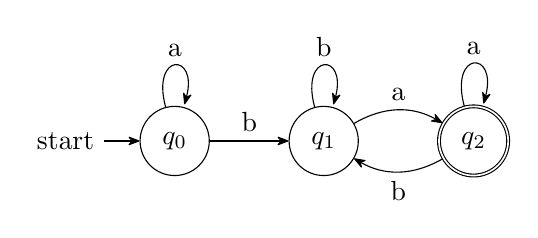
\begin{tikzpicture}[node distance = 1cm, >={Stealth[round]}]
                \node[state, initial left] (q_0) {$q_0$};
                \node[state] (q_1) [right=of q_0] {$q_1$};
                \node[state, accepting] (q_2) [right=of q_1] {$q_2$};

                \path[->]
                (q_0) edge node [above] {b} (q_1)
                (q_1) edge [bend left] node [above] {a} (q_2)
                (q_2) edge [bend left] node [below] {b} (q_1)
                (q_0) edge [loop above] node {a} ()
                (q_1) edge [loop above] node {b} ()
                (q_2) edge [loop above] node {a} ();
            \end{tikzpicture}
        \end{center}
        \caption{Module to compute $w$ contains sub. $ba$ and ends in $a$. States $p \in Q_b$}
    \end{subfigure}
    \caption{Graphical representation of the Finite Automaton of Task 9 in 2025}
\end{figure}



\stepcounter{subsection}
\subsection{Proofs of nonexistence}
We have three approaches to prove non-regularity of words.
Below is an informal guide as to how to do proofs using each of the methods and possible pitfalls.

For all of them start by assuming that $L$ is regular.

\fhlc{Cyan}{Lemma 3.3}
\setLabelNumber{lemma}{3}
\begin{lemma}[]{Unterscheidung von Wörtern}
    Sei $A$ ein EA über $\Sigma$ und $x \neq y \in \Sigma^*$ so dass $\hdelta_A (q_0, x) = \hdelta(q_0, y)$.
    Dann existiert für jedes $z \in \Sigma^*$ ein $r \in Q$, so dass $xz, yz \in \class[r]$, also gilt insbesondere
    \rmvspace
    \begin{align*}
        xz \in L(A) \Longleftrightarrow yz \in L(A)
    \end{align*}
\end{lemma}
\begin{enumerate}[noitemsep]
    \item Pick a FA $A$ over $\Sigma$ and say that $L(A) = L$
    \item Pick $|Q| + 1$ words $x$ such that $xy = w \in L$ with $|y| > 0$.
    \item State that via pigeonhole principle there exists w.l.o.g $i < j \in \{ 1, \ldots, |Q| + 1 \}$, s.t. $\hdelta_A(q_0, x_i) = \hdelta_A(q_0, x_j)$.
    \item Build contradiction by picking $z$ such that $x_i z \in L$.
    \item Then, if $z$ was picked properly, since $i < j$, we have that $x_j z \notin L$, since the lengths do not match
\end{enumerate}

\rmvspace
That is a contradiction, which concludes our proof


\fhlc{Cyan}{Pumping Lemma}
\begin{lemma}[]{Pumping-Lemma für reguläre Sprachen}
    Sei $L$ regulär. Dann existiert eine Konstante $n_0 \in \N$, so dass sich jedes Wort $w \in \word$ mit $|w| \geq n_0$ in $w = yxz$ zerlegen lässt, wobei
    \rmvspace
    \begin{multicols}{2}
        \begin{enumerate}[label=\textit{(\roman*)}]
            \item $|yx| \leq n_0$
            \item $|x| \geq 1$
            \item Für $X = \{ yx^kz \divides k\in \N \}$ \textit{entweder} $X \subseteq L$ oder $X \cap L = \emptyset$ gilt
        \end{enumerate}
    \end{multicols}
\end{lemma}

\begin{enumerate}[noitemsep]
    \item State that according to Lemma 3.4 there exists a constant $n_0$ such that $|w| \geq n_0$.
    \item Choose a word $w \in L$ that is sufficiently long to enable a sensible decomposition for the next step.
    \item Choose a decomposition, such that $|yx| = n_0$ (makes it quite easy later). Specify $y$ and $x$ in such a way that for $|y| = l$ and $|x| = m$ we have $l + m \leq n_0$
    \item According to Lemma 3.4 (ii), $m \geq 1$ and thus $|x| \geq 1$. Fix $z$ to be the suffix of $w = yxz$
    \item Then according to Lemma 3.4 (iii), fill in for $X = \{ yx^k z \divides k \in \N \}$ we have $X \subseteq L$.
    \item This will lead to a contradiction commonly when setting $k = 0$, as for a language like $0^n1^n$, we have $0^{(n_0 - m) + km}1^{n_0}$ as the word (with $n_0 - m = l$),
          which for $k = 0$ is $u= 0^{n_0 - m} 1^{n_0}$ and since $m \geq 1$, $u \notin L$ and thus by Lemma 3.4, $X \cap L = \emptyset$
\end{enumerate}


\fhlc{Cyan}{Kolmogorov Complexity}
\begin{enumerate}[noitemsep]
    \item We first need to choose an $x$ such that $L_x = \{ y | xy \in L \}$.
          If not immediately apparent, choosing $x = a^{\alpha + 1}$ for $a \in \Sigma$
          and $\alpha$ being the exponent of the exponent of the words in the language after a variable rename.
          For example, for $\{ 0^{n^2 + 2n} \divides n \in \N \}$, $\alpha(m) = m^2 + 2m$.
          Another common way to do this is for languages of the form $\{ a^n b^n \divides n \in \N \}$ to use $x = a^m$ and
          $L_{0^m} = \{ y | 0^m y \in L \} = \{ 0^j 1^{m + j} | j \in \N \}$.
    \item Find the first word $y_1 \in L_x$. In the first example, this word would be $y_1 = 0^{(m + 1)^2 \cdot 2(m + 1) - m^2 \cdot 2m + 1}$,
          or in general $a^{\alpha(m + 1) - \alpha(m) + 1}$.
          For the second example, the word would be $y_1 = 1^m$, i.e. with $j = 0$
    \item According to Theorem 3.1, there exists constant $c$ such that $K(y_k) \leq \ceil{\log_2(k + 1)} + c$. We often choose $k = 1$,
          so we have $K(y_1) \leq \ceil{\log_2(1 + 1)} + c = 1 + c$ and with $d = 1 + c$, $K(y_1) \leq d$
    \item This however leads to a contradiction, since the number of programs with length $\leq d$ is at most $2^d$ and thus finite and our set $L_x$ is infinite.
\end{enumerate}


\newpage
\fhlc{Cyan}{Minimum number of states}
To show that a language needs \textit{at least} $n$ states, use Lemma 3.3 and $n$ words. We thus again do a proof by contradiction:
\begin{enumerate}
    \item Assume that there exists FA with $|Q| < n$. We now choose $n$ words (as short as possible), as we would for non-regularity proofs using Lemma 3.3 (i.e. find some prefixes)
    \item Construct a table for the suffixes using the $n$ chosen words such that one of the words at entry $x_{ij}$ is in the language and the other is not. ($n \times n$ matrix, see below in example)
    \item Conclude that we have reached a contradiction as every field $x_{ij}$ contains a suffix such that one of the two words is in the language and the other one is not.
\end{enumerate}
\inlineex Let $L = \{ x1y \divides x \in \wordbool, y \in \{ 0, 1 \}^2 \}$. Show that any FA that accepts $L$ needs at least four states.

Assume for contradiction that there exists EA $A = (Q, \alphabetbool, \delta_A, q_0, F)$ with $|Q| < 4$.
Let's take the $4$ words $00, 01, 10, 11$. Then according to Lemma 3.3, there needs to exist a $z$ such that $xz \in L(A) \Longleftrightarrow yz \in L(A)$
with $\hdelta_A(q_0, x) = \hdelta_A(q_0, y)$ for $x, y \in \{ 00, 01, 10, 11 \}$.

This however is a contradiction, as we can find a $z$ for each of the pairs $(x, y)$, such that $xz \in L(A)$, but $yz \notin L(A)$. 
See for reference the below table (it contains suffixes $z$ fulfilling prior condition):

\begin{tables}{c|cccc}{ & $00$ & $01$ & $10$ & $11$}
              $00$      & -    & $00$ & $0$  & $0$   \\
              $01$      &      & -    & $0$  & $0$   \\
              $10$      &      &      & -    & $00$   \\
              $11$      &      &      &      & -     \\
\end{tables}
Thus, all four words have to lay in pairwise distinct states and we thus need at least $4$ states to detect this language.




\subsection{Non-determinism}
The most notable differences between deterministic and non-deterministic FA is that the transition function maps is different: $\delta: Q \times \Sigma \rightarrow \mathcal{P}(Q)$.
I.e., there can be any number of transitions for one symbol from $\Sigma$ from each state.
This is (in graphical notation) represented by arrows that have the same label going to different nodes.

It is also possible for there to not be a transition function for a certain element of the input alphabet.
In that case, regardless of state, the NFA rejects, as it ``gets stuck'' in a state and can't finish processing.

Additionally, the NFA accepts $x$ if it has at least one accepting calculation on $x$.

\stepLabelNumber{theorem}
\inlinetheorem For every NFA $M$ there exists a FA $A$ such that $L(M) = L(A)$. They are then called \bi{equivalent}


\fhlc{Cyan}{Potenzmengenkonstruktion}
States are no now sets of states of the NFA in which the NFA could be in after processing the preceding input elements and we have a special state called $q_{\text{trash}}$.

For each state, the set of states $P = \hdelta(q_0, z)$ for $|z| = n$ represents all possible states that the NFA could be in after doing the first $n$ calculations.

Correspondingly, we add new states if there is no other state that is in the same branch of the calculation tree $\mathcal{B}_M(x)$.
So, in other words, we execute BFS on the calculation tree.

\newsection
\section{Turing Machines}
\setcounter{subsection}{2}
\subsection{Representation}
Turing machines are much more capable than FA and NFA. A full definition of them can be found in the book on pages 96 - 98 (= pages 110 - 112 in the PDF).

For example, to detect a recursive language like $\{ 0^n 1^n \divides n \in \N \}$ we simply replace the left and rightmost symbol with a different one
and repeat until we only have the new symbol, at which point we accept, or there are no more $0$s or $1$s, at which point we reject.

The Turing Machines have an accepting $\qacc$ and a rejecting state $\qrej$ and a configuration is an element of
$\{ \cent \}\cdot \Gamma^* \cdot Q \cdot \Gamma^+ \cup Q \cdot \{ \cent \} \cdot \Gamma^+ \}$ with $\cdot$ being the concatenation and $\cent$ the marker of the start of the band.


\subsection{Multi-tape TM and Church's Thesis}
$k$-Tape Turing machines have $k$ extra tapes that can be written to and read from, called memory tapes. They \textit{cannot} write to the input tape.
Initially the memory tapes are empty and we are in state $q_0$.
All read/write-heads of the memory tapes can move in either direction, granted they have not reached the far left end, marked with $\cent$.

As with normal TMs, the Turing Machine $M$ accepts $w$ if and only if $M$ reaches the state $\qacc$ and rejects if it does not terminate or reaches the state $\qrej$

\inlinelemma There exists and equivalent $1$-Tape-TM for every TM.

\inlinelemma There exists an equivalent TM for each Multi-tape TM.


Church's Thesis states that the Turing Machines are a formalization of the term ``Algorithm''.
It is the only axiom specific to Computer Science.

All the words that can be accepted by a Turing Machine are elements of $\mathcal{L}_{RE}$ and are called \bi{recursively enumerable}.


\subsection{Non-Deterministic Turin Machines}
The same ideas as with NFA apply here. The transition function also maps into the power set:
\rmvspace
\begin{align*}
    \delta : (Q - \{ \qacc, \qrej \}) \times \Gamma \rightarrow \mathcal{P}(Q \times \Gamma \times \{ L, R, N \})
\end{align*}

Again, when constructing a normal TM from a NTM (which is not required at the Midterm, or any other exam for that matter in this course),
we again apply BFS to the NTM's calculation tree.

\stepLabelNumber{theorem}
\inlinetheorem For an NTM $M$ exists a TM $A$ s.t. $L(M) = L(A)$ and if $M$ doesn't contain infinite calculations on words of $(L(M))^C$, then $A$ always stops.

\newsection
\section{Computability}
\stepcounter{subsection}
\subsection{Diagonalization}
The \bi{set of binary encodings of all TMs} is denoted $\text{KodTM}$ and $\text{KodTM} \subseteq \wordbool$ and the upper bound of the cardinality is $|\wordbool|$,
as there are infinitely many TMs.

Below is a list of countable objects. They all have corresponding Lemmas in the script, but omitted here:
\drmvspace
\begin{multicols}{4}
    \begin{itemize}
        \item $\word$ for any $\Sigma$
        \item $\text{KodTM}$
        \item $\N \times \N$
        \item $\Q^+$
    \end{itemize}
\end{multicols}

\rmvspace
\drmvspace
The following objects are uncountable: $[0, 1]$, $\R$, $\mathcal{P}(\wordbool)$

\inlinecorollary $|\text{KodTM}| < |\mathcal{P}(\wordbool)|$ and thus there exist infinitely many not recursively enumerable languages over $\alphabetbool$

\fhlc{Cyan}{Proof of $L$ (not) recursively enumerable}

Proving that a language \textit{is} recursively enumerable is as easy as providing a Turing Machine that accepts it.

Proving that a language is \textit{not} recursively enumerable is a bit harder. For it, let $d_{ij} = 1 \Longleftrightarrow M_i$ accepts $w_j$.

As an example, we'll use the following language

Assume towards contradiction that $L_\text{diag} \in \mathcal{L}_{RE}$. Let 
\begin{align*}
    L_{\text{diag}} & = \{ w \in \wordbool \divides w = w_i \text{ for an } i \in \N - \{ 0 \} \text{ and $M_i$ does not accept } w_i \} \\
                    & = \{ w \in \wordbool \divides w = w_i \text{ for an } i \in \N - \{ 0 \} \text{ and } d_{ii} = 0\}
\end{align*}
Thus assume that, $L_\text{diag} = L(M)$ for a Turing Machine $M$.
Since $M$ is a Turing Machine in the canonical ordering of all Turing Machines, so there exists an $i \in \N - \{ 0 \}$, such that $M = M_i$.

This however leads to a contradiction, as $w_i \in L_\text{diag} \Longleftrightarrow d_{ii} = 0 \Longleftrightarrow w_i \notin L(M_i)$.

In other words, $w_i$ is in $L_\text{diag}$ if and only if $w_i$ is not in $L(M_i)$, which contradicts our statement above.

\setLabelNumber{theorem}{3}
\inlinetheorem $L_\text{diag} \notin \mathcal{L}_{RE}$




\end{document}
